\documentclass[tikz, border=10pt]{standalone}
\usepackage{helvet}
\renewcommand{\familydefault}{\sfdefault}
\usetikzlibrary{shapes.geometric, arrows.meta, positioning, fit, calc, backgrounds}

\begin{document}
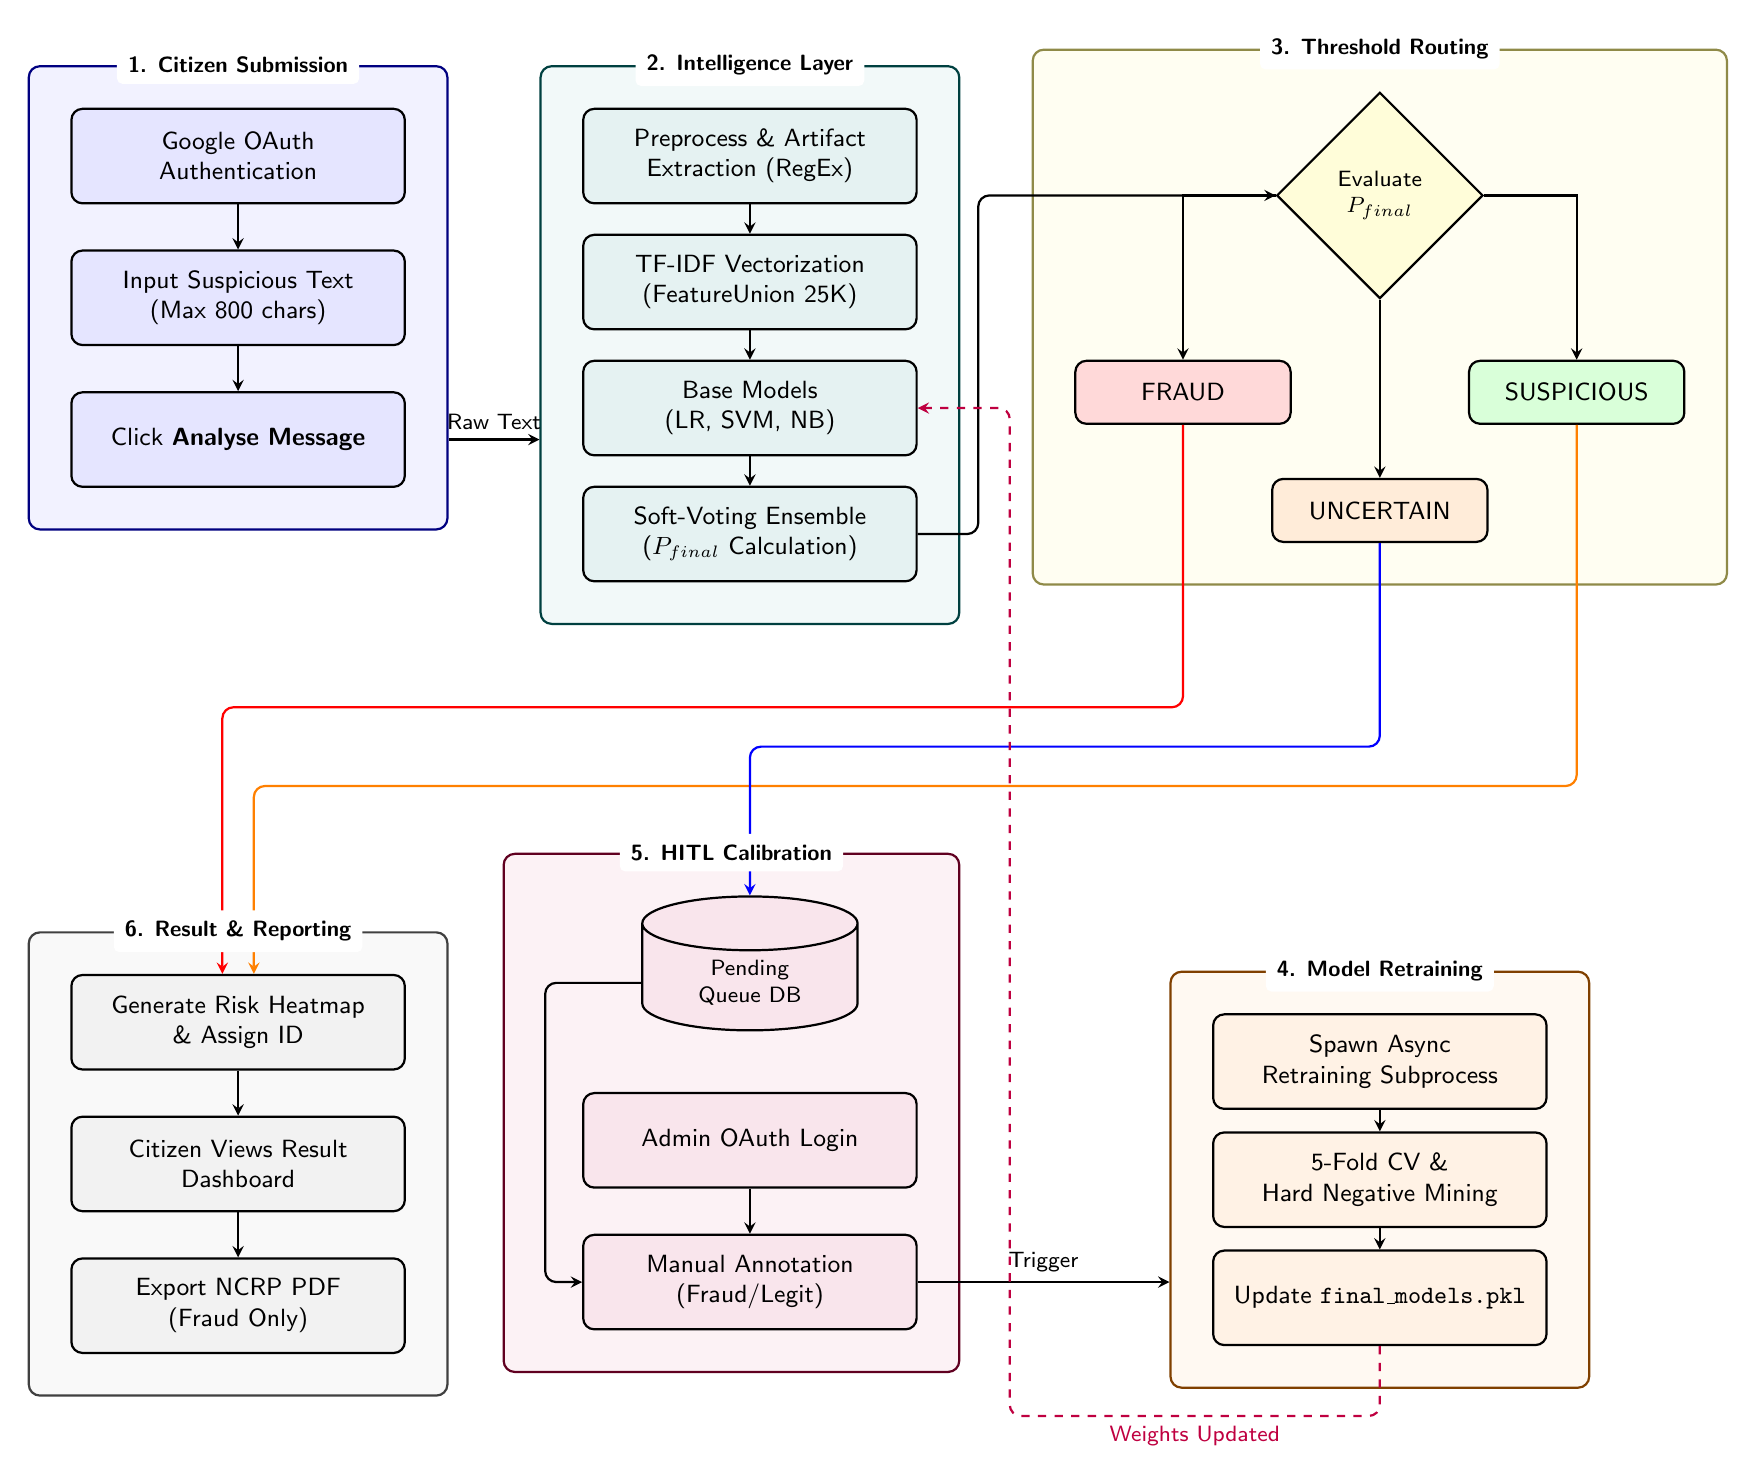
\begin{tikzpicture}[
    node distance=1.5cm and 1.5cm,
    process/.style={rectangle, rounded corners=4pt, draw=black, thick, text=black, fill=white, text width=4.0cm, align=center, minimum height=1.2cm, font=\small},
    decision/.style={diamond, draw=black, thick, fill=white, text=black, text width=2.0cm, align=center, inner sep=0pt, font=\footnotesize},
    database/.style={cylinder, shape border rotate=90, draw=black, thick, aspect=0.25, text=black, fill=white, text width=2.5cm, align=center, minimum height=1.5cm, font=\footnotesize},
    arrow/.style={->, thick, >=stealth, draw=black},
    feedback/.style={->, dashed, thick, >=stealth, draw=black},
    blockLabel/.style={rectangle, fill=white, text=black, font=\bfseries\footnotesize, rounded corners=2pt, inner sep=4pt}
]

% Define Coordinates
\def\xColA{0}
\def\xColB{6.5}
\def\xColC{14.5}
\def\yRowA{0}
\def\yRowB{-11}

% ================= BLOCK 1 =================
\node[process, fill=blue!10] (b1_1) at (\xColA, \yRowA) {Google OAuth Authentication};
\node[process, fill=blue!10] (b1_2) at (\xColA, \yRowA-1.8) {Input Suspicious Text\\(Max 800 chars)};
\node[process, fill=blue!10] (b1_3) at (\xColA, \yRowA-3.6) {Click \textbf{Analyse Message}};

\draw[arrow] (b1_1) -- (b1_2);
\draw[arrow] (b1_2) -- (b1_3);

\begin{scope}[on background layer]
    \node[draw=blue!50!black, thick, rounded corners, inner sep=15pt, fill=blue!5, fit=(b1_1) (b1_3)] (box1) {};
\end{scope}

% ================= BLOCK 2 =================
\node[process, fill=teal!10] (b2_1) at (\xColB, \yRowA) {Preprocess \& Artifact\\Extraction (RegEx)};
\node[process, fill=teal!10] (b2_2) at (\xColB, \yRowA-1.6) {TF-IDF Vectorization\\(FeatureUnion 25K)};
\node[process, fill=teal!10] (b2_3) at (\xColB, \yRowA-3.2) {Base Models\\(LR, SVM, NB)};
\node[process, fill=teal!10] (b2_4) at (\xColB, \yRowA-4.8) {Soft-Voting Ensemble\\($P_{final}$ Calculation)};

\draw[arrow] (b2_1) -- (b2_2);
\draw[arrow] (b2_2) -- (b2_3);
\draw[arrow] (b2_3) -- (b2_4);

\begin{scope}[on background layer]
    \node[draw=teal!50!black, thick, rounded corners, inner sep=15pt, fill=teal!5, fit=(b2_1) (b2_4)] (box2) {};
\end{scope}

% Connect Block 1 to Block 2
\draw[arrow] (box1.east |- b1_3) -- (box2.west |- b1_3) node[midway, above, font=\footnotesize] {Raw Text};

% ================= BLOCK 3 =================
\node[decision, fill=yellow!15] (b3_1) at (\xColC, \yRowA-0.5) {Evaluate\\$P_{final}$};
\node[process, text width=2.5cm, minimum height=0.8cm, fill=red!15] (b3_2) at (\xColC-2.5, \yRowA-3) {FRAUD};
\node[process, text width=2.5cm, minimum height=0.8cm, fill=orange!15] (b3_3) at (\xColC, \yRowA-4.5) {UNCERTAIN};
\node[process, text width=2.5cm, minimum height=0.8cm, fill=green!15] (b3_4) at (\xColC+2.5, \yRowA-3) {SUSPICIOUS};

\draw[arrow] (b3_1.west) -| (b3_2.north);
\draw[arrow] (b3_1.south) -- (b3_3.north);
\draw[arrow] (b3_1.east) -| (b3_4.north);

\begin{scope}[on background layer]
    \node[draw=yellow!50!black, thick, rounded corners, inner sep=15pt, fill=yellow!5, fit=(b3_1) (b3_2) (b3_3) (b3_4)] (box3) {};
\end{scope}

% Connect Block 2 to Block 3
\draw[arrow, rounded corners] (b2_4.east) -- (9.4, \yRowA-4.8) -- (9.4, \yRowA-0.5) -- (b3_1.west);

% ================= BLOCK 4 =================
\node[process, fill=gray!10] (b4_1) at (\xColA, \yRowB) {Generate Risk Heatmap\\\& Assign ID};
\node[process, fill=gray!10] (b4_2) at (\xColA, \yRowB-1.8) {Citizen Views Result\\Dashboard};
\node[process, fill=gray!10] (b4_3) at (\xColA, \yRowB-3.6) {Export NCRP PDF\\(Fraud Only)};

\draw[arrow] (b4_1) -- (b4_2);
\draw[arrow] (b4_2) -- (b4_3);

\begin{scope}[on background layer]
    \node[draw=gray!50!black, thick, rounded corners, inner sep=15pt, fill=gray!5, fit=(b4_1) (b4_3)] (box4) {};
\end{scope}

% ================= BLOCK 5 =================
\node[database, fill=purple!10] (b5_1) at (\xColB, \yRowB+0.5) {Pending\\Queue DB};
\node[process, fill=purple!10] (b5_2) at (\xColB, \yRowB-1.5) {Admin OAuth Login};
\node[process, fill=purple!10] (b5_3) at (\xColB, \yRowB-3.3) {Manual Annotation\\(Fraud/Legit)};

\draw[arrow, rounded corners] (b5_1.west) -| (\xColB-2.6, \yRowB-1.4) |- (b5_3.west);
\draw[arrow] (b5_2) -- (b5_3);

\coordinate (b5_curve) at (\xColB-2.6, \yRowB-1.4);
\begin{scope}[on background layer]
    \node[draw=purple!50!black, thick, rounded corners, inner sep=15pt, fill=purple!5, fit=(b5_1) (b5_3) (b5_curve)] (box5) {};
\end{scope}

% ================= BLOCK 6 =================
\node[process, fill=orange!10] (b6_1) at (\xColC, \yRowB-0.5) {Spawn Async\\Retraining Subprocess};
\node[process, fill=orange!10] (b6_2) at (\xColC, \yRowB-2.0) {5-Fold CV \&\\Hard Negative Mining};
\node[process, fill=orange!10] (b6_3) at (\xColC, \yRowB-3.5) {Update \texttt{final\_models.pkl}};

\draw[arrow] (b6_1) -- (b6_2);
\draw[arrow] (b6_2) -- (b6_3);

\begin{scope}[on background layer]
    \node[draw=orange!50!black, thick, rounded corners, inner sep=15pt, fill=orange!5, fit=(b6_1) (b6_3)] (box6) {};
\end{scope}
% label moved to end

% ================= INTER-BLOCK ARROWS =================

% Routing to Results (Legit and Fraud)
\draw[arrow, draw=red, rounded corners] (b3_2.south) -- (\xColC-2.5, -7.0) -- (-0.2, -7.0) -- ([xshift=-0.2cm]b4_1.north);
\draw[arrow, draw=orange, rounded corners] (b3_4.south) -- (\xColC+2.5, -8.0) -- (0.2, -8.0) -- ([xshift=0.2cm]b4_1.north);

% Routing to HITL (Uncertain)
\draw[arrow, draw=blue, rounded corners] (b3_3.south) -- (\xColC, -7.5) -- (\xColB, -7.5) -- (b5_1.north);

% HITL to Retraining
\draw[arrow] (b5_3.east) -- (box6.west |- b5_3.east) node[midway, above, font=\footnotesize] {Trigger};

% Retraining Feedback Loop
\draw[feedback, draw=purple, rounded corners] (b6_3.south) -- (\xColC, -16.0) -- (9.8, -16.0) node[midway, below, text=purple, font=\footnotesize] {Weights Updated} -- (9.8, -3.2) -- (b2_3.east);

% ================= LABELS DRAWN LAST =================
\node[blockLabel] at (box1.north) {1. Citizen Submission};
\node[blockLabel] at (box2.north) {2. Intelligence Layer};
\node[blockLabel] at (box3.north) {3. Threshold Routing};
\node[blockLabel] at (box4.north) {6. Result \& Reporting};
\node[blockLabel] at (box5.north) {5. HITL Calibration};
\node[blockLabel] at (box6.north) {4. Model Retraining};

\end{tikzpicture}
\end{document}
